% Figures and tables, each legend on the same page as its figure (npj requirement).

\begin{table}[t]
\caption{\textbf{Cohorts.} DR is graded on the international 5-grade scale
in every corpus. No external image was used for training, model selection or
threshold fitting. Messidor-2 and DDR were used from public 512-pixel mirrors; SUSTech-SYSU's
grade-0 images are of healthy volunteers without diabetes, and its 68 laser-scar images carry no grade.}\label{tab:cohorts}
\centering\footnotesize\setlength{\tabcolsep}{3pt}
\begin{tabular}{@{}p{2.3cm}p{3.1cm}p{2.4cm}p{2.3cm}p{2.7cm}@{}}
\toprule
Role & Corpus & Origin & Images & Grading \\
\midrule
Development & IDRiD & India & 516 & 3 graders (published grading) \\
 & Messidor-2 & France & 1,744 & adjudicated by 3 specialists \\
Pretraining; EyePACS models & EyePACS 2015 & USA & 35,126 & single grader per image \\
External & APTOS 2019 & India & 3,662 & single grader \\
 & DDR & China, 147 hospitals & 12,522 & 7 graders \\
 & DeepDRiD (regular) & China, 3 diabetes screening programmes & 2,000 (500 patients) & doctor annotations (challenge release) \\
 & SUSTech-SYSU & China, Guangdong; case--control & 1,151 graded of 1,219 & 2 ophthalmologists, adjudicated \\
Reverse direction & APTOS $\rightarrow$ Messidor-2, IDRiD &  & 3,662 $\rightarrow$ 2,260 & as above \\
\bottomrule
\end{tabular}
\end{table}


\begin{figure}[p]
\centering
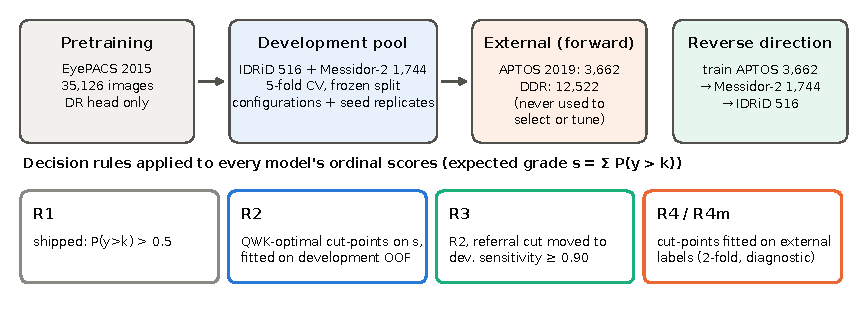
\includegraphics[width=\textwidth]{figures/fig1_design.pdf}
\caption{\textbf{Study design.} Models were pretrained on EyePACS, developed on a pooled IDRiD
and Messidor-2 set under a frozen 5-fold split, and evaluated without any further tuning on
APTOS 2019 and DDR; a separate model trained on APTOS with the same recipe was evaluated on
Messidor-2 and IDRiD (reverse direction). Every model's ordinal outputs were decoded under the
same five decision rules: R1, the shipped default; R2 and R3, deployable rules fitted on
development predictions; and R4/R4m, diagnostic rules fitted on the external labels by two-fold
cross-fitting, which bound what local recalibration can recover and are never reported as
performance.}
\label{fig:design}
\end{figure}

\begin{figure}[p]
\centering
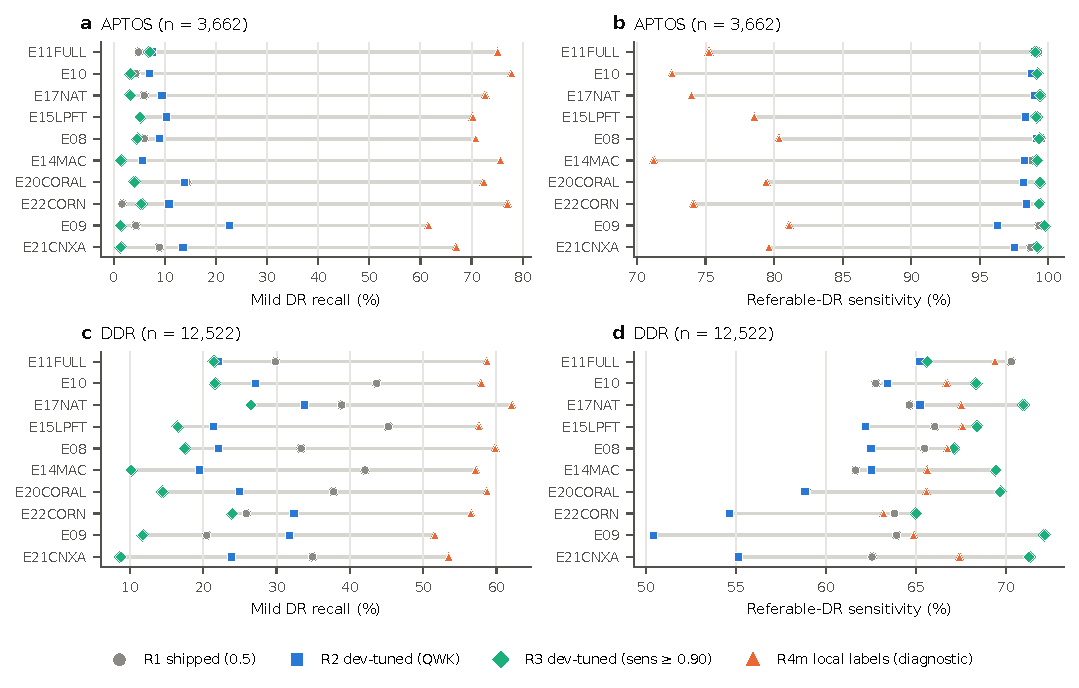
\includegraphics[width=\textwidth]{figures/fig2_rules.pdf}
\caption{\textbf{The decision rule moves external mild-grade recall and referral sensitivity
more than the choice of model.} Each row is one development model (sorted by development QWK
at matched calibration); markers show the same model's external metric under the four
decision rules. \textbf{a},\textbf{b}, APTOS 2019; \textbf{c},\textbf{d}, DDR. Mild recall
under the shipped rule is uniformly low and is restored by external cut-points (R4m) in every
model, without retraining; development-fitted rules (R2, R3) do not restore it. The spread
across models under any fixed rule is small compared with the spread across rules within a
model. Referral sensitivity under R4m falls because mild DR is not a referable grade.}
\label{fig:rules}
\end{figure}

\begin{figure}[p]
\centering
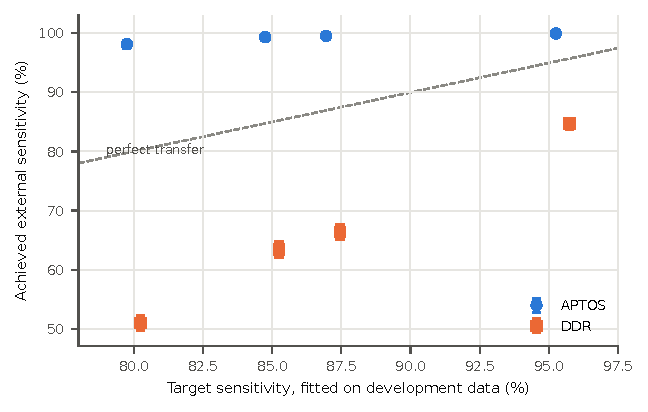
\includegraphics[width=0.75\textwidth]{figures/fig3_transfer.pdf}
\caption{\textbf{Thresholds fitted on development data overshoot on new populations.} A
referral threshold on $P(\mathrm{grade}\geq2)$ was fitted on the development out-of-fold
predictions of the reference model to reach each target sensitivity (x-axis), then applied
unchanged to APTOS and DDR. Points show the achieved external sensitivity with 95\% bootstrap
intervals; the diagonal is perfect transfer. Targets: 80\%; 85\% (the pre-specified
superiority endpoint of the first autonomous pivotal trial); 87.2\% (that trial's achieved
sensitivity); 95.5\% (a reported pivotal-trial sensitivity).}
\label{fig:transfer}
\end{figure}

\begin{figure}[p]
\centering
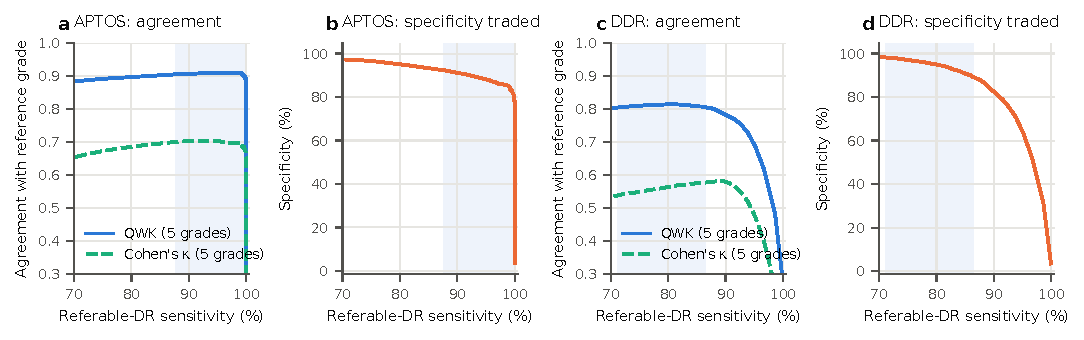
\includegraphics[width=\textwidth]{figures/fig4_frontier.pdf}
\caption{\textbf{Agreement statistics cannot see the referral operating point, and
development-fitted thresholds do not transfer.} \textbf{a},\textbf{c}, QWK and Cohen's
$\kappa$ of the selected model as the referral cut-point is swept with the other cut-points held
at their QWK-optimal values, plotted against the referable-DR sensitivity it produces, on APTOS
(\textbf{a}) and DDR (\textbf{c}). The shaded band contains every operating point whose QWK is
within 0.01 of the maximum. \textbf{b},\textbf{d}, the specificity that the same sweep trades
for sensitivity. Inside the band the referral decision changes by tens of points while the
grading statistic does not.}
\label{fig:frontier}
\end{figure}

\begin{figure}[p]
\centering
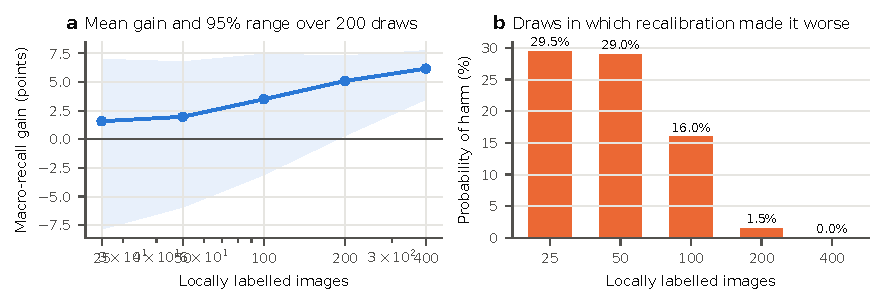
\includegraphics[width=0.85\textwidth]{figures/fig5_recalibration.pdf}
\caption{\textbf{How many locally labelled images recalibration needs.} Cut-points were fitted
(maximising macro-averaged recall) on $n$ APTOS images drawn at random and evaluated on the
remaining images, 200 draws per size. \textbf{a}, mean gain in macro-averaged recall over the
shipped rule with the 2.5th--97.5th percentile range of draws. \textbf{b}, probability that a
draw ends worse than the shipped rule. The mean gain is positive at every size, but below 100
images roughly one recalibration in four does harm.}
\label{fig:recal}
\end{figure}

\begin{figure}[p]
\centering
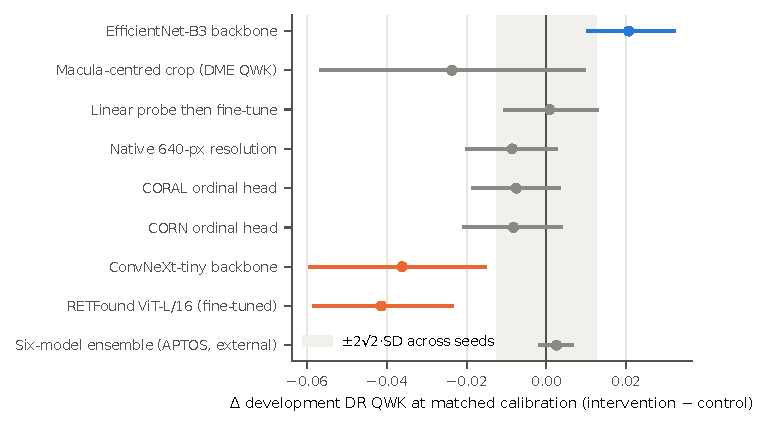
\includegraphics[width=0.8\textwidth]{figures/fig6_forest.pdf}
\caption{\textbf{Pre-registered interventions on the model.} Difference in development DR QWK
(intervention minus control) at matched calibration with 95\% paired-bootstrap intervals; the
macula-centred crop was registered on the DME head (DME QWK shown) and the ensemble on the
external set (APTOS QWK shown). The grey band is $\pm2\sqrt{2}$ standard deviations of the
matched development QWK across five seeds of the reference configuration, the pre-registered
yardstick for a difference beyond seed noise. Blue, pre-registered improvement confirmed;
orange, interval excludes zero in the unfavourable direction; grey, indistinguishable.}
\label{fig:forest}
\end{figure}

\begin{table}[t]
\caption{\textbf{Decision-rule reanalysis of a published model family (ORDER-DR,
APTOS$\rightarrow$Messidor-2).} Mean $\pm$ s.d. over the authors' three seeds, computed
from their released image-level probabilities on 1,744 Messidor-2 images
(270 mild). For ORDER-DR the R2 row uses the authors' own fusion and cut-points
and reproduces their reported result. R4/R4m use external labels (two-fold cross-fitting)
and are diagnostic bounds, not performance claims.}\label{tab:orderdr}
\centering\footnotesize
\begin{tabular}{@{}llccccc@{}}
\toprule
Model & Rule & QWK & Mild recall (\%) & Mild F1 & Ref.\ sens.\ (\%) & Ref.\ spec.\ (\%) \\
\midrule
CB-384 & argmax & 0.500 $\pm$ 0.018 & 2.0 & 0.027 & 32.8 & 99.5 \\
 & validation-fitted (published) & 0.544 $\pm$ 0.029 & 2.5 & 0.035 & 38.2 & 99.0 \\
 & external, QWK & 0.672 $\pm$ 0.030 & 27.8 & 0.231 & 55.1 & 95.4 \\
 & external, macro-recall & 0.614 $\pm$ 0.060 & 38.4 & 0.255 & 72.6 & 85.2 \\
\addlinespace
LORS-384 & argmax & 0.531 $\pm$ 0.014 & 3.5 & 0.049 & 36.3 & 98.9 \\
 & validation-fitted (published) & 0.570 $\pm$ 0.023 & 2.7 & 0.041 & 42.8 & 98.7 \\
 & external, QWK & 0.683 $\pm$ 0.045 & 30.5 & 0.245 & 55.9 & 96.1 \\
 & external, macro-recall & 0.677 $\pm$ 0.046 & 36.5 & 0.285 & 67.6 & 91.3 \\
\addlinespace
Swin-T & argmax & 0.552 $\pm$ 0.045 & 5.2 & 0.062 & 35.4 & 96.9 \\
 & validation-fitted (published) & 0.564 $\pm$ 0.026 & 3.3 & 0.045 & 43.2 & 96.2 \\
 & external, QWK & 0.674 $\pm$ 0.022 & 13.0 & 0.147 & 64.8 & 93.8 \\
 & external, macro-recall & 0.629 $\pm$ 0.041 & 30.2 & 0.233 & 75.0 & 88.9 \\
\addlinespace
ORDER-DR & argmax & 0.509 $\pm$ 0.017 & 2.7 & 0.040 & 34.1 & 99.2 \\
 & validation-fitted (published) & 0.642 $\pm$ 0.036 & 50.5 & 0.277 & 39.8 & 99.1 \\
 & external, QWK & 0.676 $\pm$ 0.025 & 24.2 & 0.212 & 56.7 & 95.4 \\
 & external, macro-recall & 0.638 $\pm$ 0.049 & 42.0 & 0.284 & 70.0 & 88.8 \\
\bottomrule
\end{tabular}
\end{table}

\begin{table}[t]
\caption{\textbf{Matched calibration changes model comparisons.} Differences (first minus
second) with 95\% paired-bootstrap intervals at the shipped rule and with both models'
cut-points refitted by the same procedure (external rows: R4, two-fold cross-fitted on
APTOS labels; development rows: fold-wise cross-fitted). $^\ast$Interval excludes zero.
$^\dagger$Under random-half cross-fitting the matched difference is significant; under
fold-wise cross-fitting it is not (Supplementary Note~3).}\label{tab:record}
\centering\footnotesize
\begin{tabular}{@{}p{5.4cm}p{2.9cm}p{2.9cm}l@{}}
\toprule
Comparison & Shipped rule & Matched calibration & Verdict \\
\midrule
EfficientNet-B3 vs DenseNet121, APTOS QWK & +0.0059 [+0.0007, +0.0110] & +0.0032 [$-$0.0020, +0.0083] & advantage dissolves \\
\quad recall, moderate (points) & +1.4 & +4.0$^\ast$ & significance changes \\
\quad recall, severe (points) & $-$1.0 & $-$10.3$^\ast$ & significance changes \\
\quad recall, proliferative (points) & +8.1$^\ast$ & +6.8$^\ast$ & persists \\
LP-FT vs fine-tuning, development accuracy (points) & $-$5.54 [$-$7.48, $-$3.54] & +1.95 [+0.18, +3.72] & reverses \\
EfficientNet-B3 vs DenseNet121, development QWK & +0.0202 [+0.0071, +0.0329] & +0.0207 [+0.0105, +0.0320] & survives \\
Image source (E12), moderate recall (points)$^\dagger$ & $-$6.9 [$-$12.1, $-$2.1] & +0.4 [$-$5.7, +6.1] & procedure-dependent \\
\bottomrule
\end{tabular}
\end{table}

